\documentclass{article}
\usepackage{graphicx}
\usepackage[margin=1in]{geometry}
\usepackage{listings}
\usepackage{amsmath}
\usepackage{mathtools}

\begin{document}

\title{CS102: Week 11}

\maketitle
\section*{Extend the Point Class}
Using the point class described in class, add the following methods:
\begin{description}
	\item [void display()] prints out "Point(\textit{x},\textit{y})"
	\item[int quadrant()] returns the quadrant (1,2,3,4) that the Point object lies in\\
	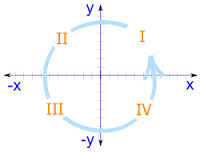
\includegraphics[width=.25\textwidth]{images}
	\item[int above(Point P)] checks if the point calling the function is above the point P.\\ 
                                                   For example, given P1.above(P2), the method should return:
		\begin{description}
			\item[1] $\frac{P1}{P2}$
			\item[0] P1     P2
			\item[-1] $\frac{P2}{P1}$
		\end{description}
	\item

	\item[int toRight(Point P)] checks if the point calling the function is to the right of the point P.\\ 
                                                   For example, given P1.toRight(P2), the method should return:
		\begin{description}
			\item[1]  P2    P1
			\item[0]  P\rlap{1}{2}
			\item[-1] P1    P2
		\end{description}
	
\end{description}
\pagebreak

\section*{Line Functions}
Write a program that includes and uses the following functions:
\begin{description}
	\item[double slope(Point P1, Point P2)] compute the slope of the line that intersects P1 and P2
	\item[double intercept(Point P1, Point P2)] compute the y intercept of the line that intersects P1 and P2
\end{description}

\section*{Line Class}
Write a line class using the following declaration and a program to test the class. 
\begin{lstlisting}{c++}
class Line{
	public: 
		double slope;
		double intercept;
		Line(Point P1, Point P2);
		//returns true if the line intersects the point
		bool intersects(Point P);
};
\end{lstlisting}

\end{document}